
\chapter{Seguridad Eléctrica en Sistemas Fotovoltaicos}
\label{sec:seguridad}

\section{Introducción}

El funcionamiento de un sistema fotovoltaico supone la existencia
de ciertas situaciones que pueden ser peligrosas para las personas
o dañinas para los equipos. En términos generales, estas situaciones
pueden ser analizadas con los conceptos y herramientas de uso común
en la ingeniería eléctrica. No obstante, las peculiaridades de la
tecnología fotovoltaica merecen un análisis especial en el contexto
de la seguridad eléctrica. Este análisis será realizado en tres apartados
principales. En primer lugar se estudiará el riesgo para las personas
y los mecanismos de protección asociados. A continuación se hará lo
propio con las posibilidades de accidente y métodos de protección
para los equipos del sistema. Para cerrar el capítulo se expondrán
los métodos de elección de los diferentes dispositivos de protección
aplicados a un sistema fotovoltaico.

Durante el desarrollo de este capítulo se hará continua referencia
a un documento básico en la práctica de la ingeniería eléctrica en
España: el Reglamento Electrotécnico de Baja Tensión (REBT) \cite{RD_842_2002}.
Esta normativa, aprobada por Real Decreto en el año 2002, consta de
29 artículos que son desarrollados en un conjunto de 51 Instrucciones
Técnicas Complementarias (ITC-BT) y acompañadas por varias guías de
aplicación. Es reseñable que ni en los artículos ni en las ITC-BT
aparece referencia alguna a los sistemas fotovoltaicos, lo que, en
algunos casos particulares, dificulta la aplicación de este REBT a
la ingeniería fotovoltaica.


\subsection{Definiciones}

Para el desarrollo posterior nos serán útiles algunas definiciones
recogidas en la ITC-BT-01:
\begin{description}
\item [{Contacto~Directo:}] contacto de personas o animales con partes
activas de los materiales y equipos.
\item [{Contacto~Indirecto:}] contacto de personas o animales con partes
que se han puesto bajo tensión como resultado de un fallo de aislamiento.
\item [{Partes~Activas:}] Conductores y piezas conductoras bajo tensión
en servicio normal. Incluyen el conductor neutro o compensador y las
partes a ellos conectadas.
\item [{Masa:}] Conjunto de las partes metálicas de un aparato que, en
condiciones normales, están aisladas de las partes activas.
\item [{Tierra:}] Masa conductora de la tierra en la que el potencial eléctrico
en cada punto se toma, convencionalmente, igual a cero.
\item [{Toma~de~tierra:}] Electrodo, o conjunto de electrodos, en contacto
con el suelo y que asegura la conexión eléctrica con el mismo.
\item [{Material~de~clase~0:}] Material en el cual la protección contra
el choque eléctrico se basa en el aislamiento principal; lo que implica
que no existe ninguna disposición prevista para la conexión de las
partes activas accesibles, si las hay, a un conductor de protección
que forme parte del cableado fijo de la instalación. La protección
en caso de defecto en el aislamiento principal depende del entorno.
\item [{Material~de~clase~I:}] la protección contra el choque eléctrico
no se basa únicamente en el aislamiento principal, sino que comporta
una medida de seguridad complementaria en forma de medios de conexión
de las partes conductoras accesibles a un conductor de protección
puesto a tierra, que forma parte del cableado fijo de la instalación,
de forma tal que las partes conductoras accesibles no puedan presentar
tensiones peligrosas.
\item [{Material~de~clase~II:}] la protección comporta medidas de seguridad
complementarias, tales como el doble aislamiento o aislamiento reforzado.
Estas medidas no suponen la utilización de puesta a tierra para la
protección y no dependen de las condiciones de la instalación. Este
material debe estar alimentado por cables con doble aislamiento o
con aislamiento reforzado.
\item [{Material~de~clase~III:}] la protección no se basa en la alimentación
a muy baja tensión y en el cual no se producen tensiones superiores
a 50 V en c.a. ó a 75 V en c.c.
\item [{Tensión~de~contacto:}] Tensión que aparece entre partes accesibles
simultáneamente, al ocurrir un fallo de aislamiento. Por convenio
este término sólo se utiliza en relación con la protección contra
contactos indirectos. En ciertos casos el valor de la tensión de contacto
puede resultar influido notablemente por la impedancia que presenta
la persona en contacto con esas partes.
\item [{Tensión~de~defecto:}] Tensión que aparece a causa de un defecto
de aislamiento, entre dos masas, entre una masa y un elemento conductor,
o entre una masa y una toma de tierra de referencia, es decir, un
punto en el que el potencial no se modifica al quedar la masa en tensión.
\end{description}
Para los esquemas de conexión a tierra se emplea una codificación
basada en dos letras:
\begin{description}
\item [{Primera~letra:}] conexión de alimentación y tierra.

\begin{description}
\item [{T=}] conexión directa de un punto de alimentación a tierra.
\item [{I=}] aislamiento de todas las partes activas respecto a tierra.
\end{description}
\item [{Segunda~letra:}] conexión de masas con tierra.

\begin{description}
\item [{T=}] masas conectadas directamente a tierra, independientemente
de la conexión de alimentación.
\item [{N=}] masas conectadas directamente al punto de alimentación puesto
a tierra (en alterna, normalmente el neutro).
\end{description}
\end{description}
Con esta codificación, los posibles esquemas de conexión a tierra
tienen la siguiente nomenclatura:
\begin{description}
\item [{TT:}] un conductor (en alterna, el neutro) puesto a tierra y masas
a tierra, pero de forma independiente. 
\item [{TN:}] un conductor (en alterna, el neutro) puesto a tierra, y masas
conectadas al neutro (directamente o a través de un conductor de protección).
\item [{IT:}] todos los conductores activos aislados de tierra, y masas
conectadas a tierra. 
\end{description}
El esquema TT es el empleado por las instalaciones receptoras en una
red de distribución pública de Baja Tensión (BT). En general, es el
esquema que debe adoptarse a la salida de los inversores de los Sistemas
Fotovoltaicos Conectados a Red (SFCR). El esquema IT es el habitual
en el generador fotovoltaico de los SFCR europeos. Es muy común referirse
al esquema IT con la denominación de configuración flotante del generador.


\section{Protección de las personas}


\subsection{Efectos de la corriente eléctrica sobre el cuerpo humano}

El efecto que produce la corriente eléctrica sobre el cuerpo humano
depende de su intensidad y del tiempo de duración, tal y como se observa
en la figura \ref{fig:EfectoCorriente}. Independientemente de la
duración hasta $\SI{10}{\milli\ampere}$ no genera efectos peligrosos
(calambres) pero por encima de $\SI{500}{\milli\ampere}$ puede producir
fibrilación muscular.

%
\begin{figure}
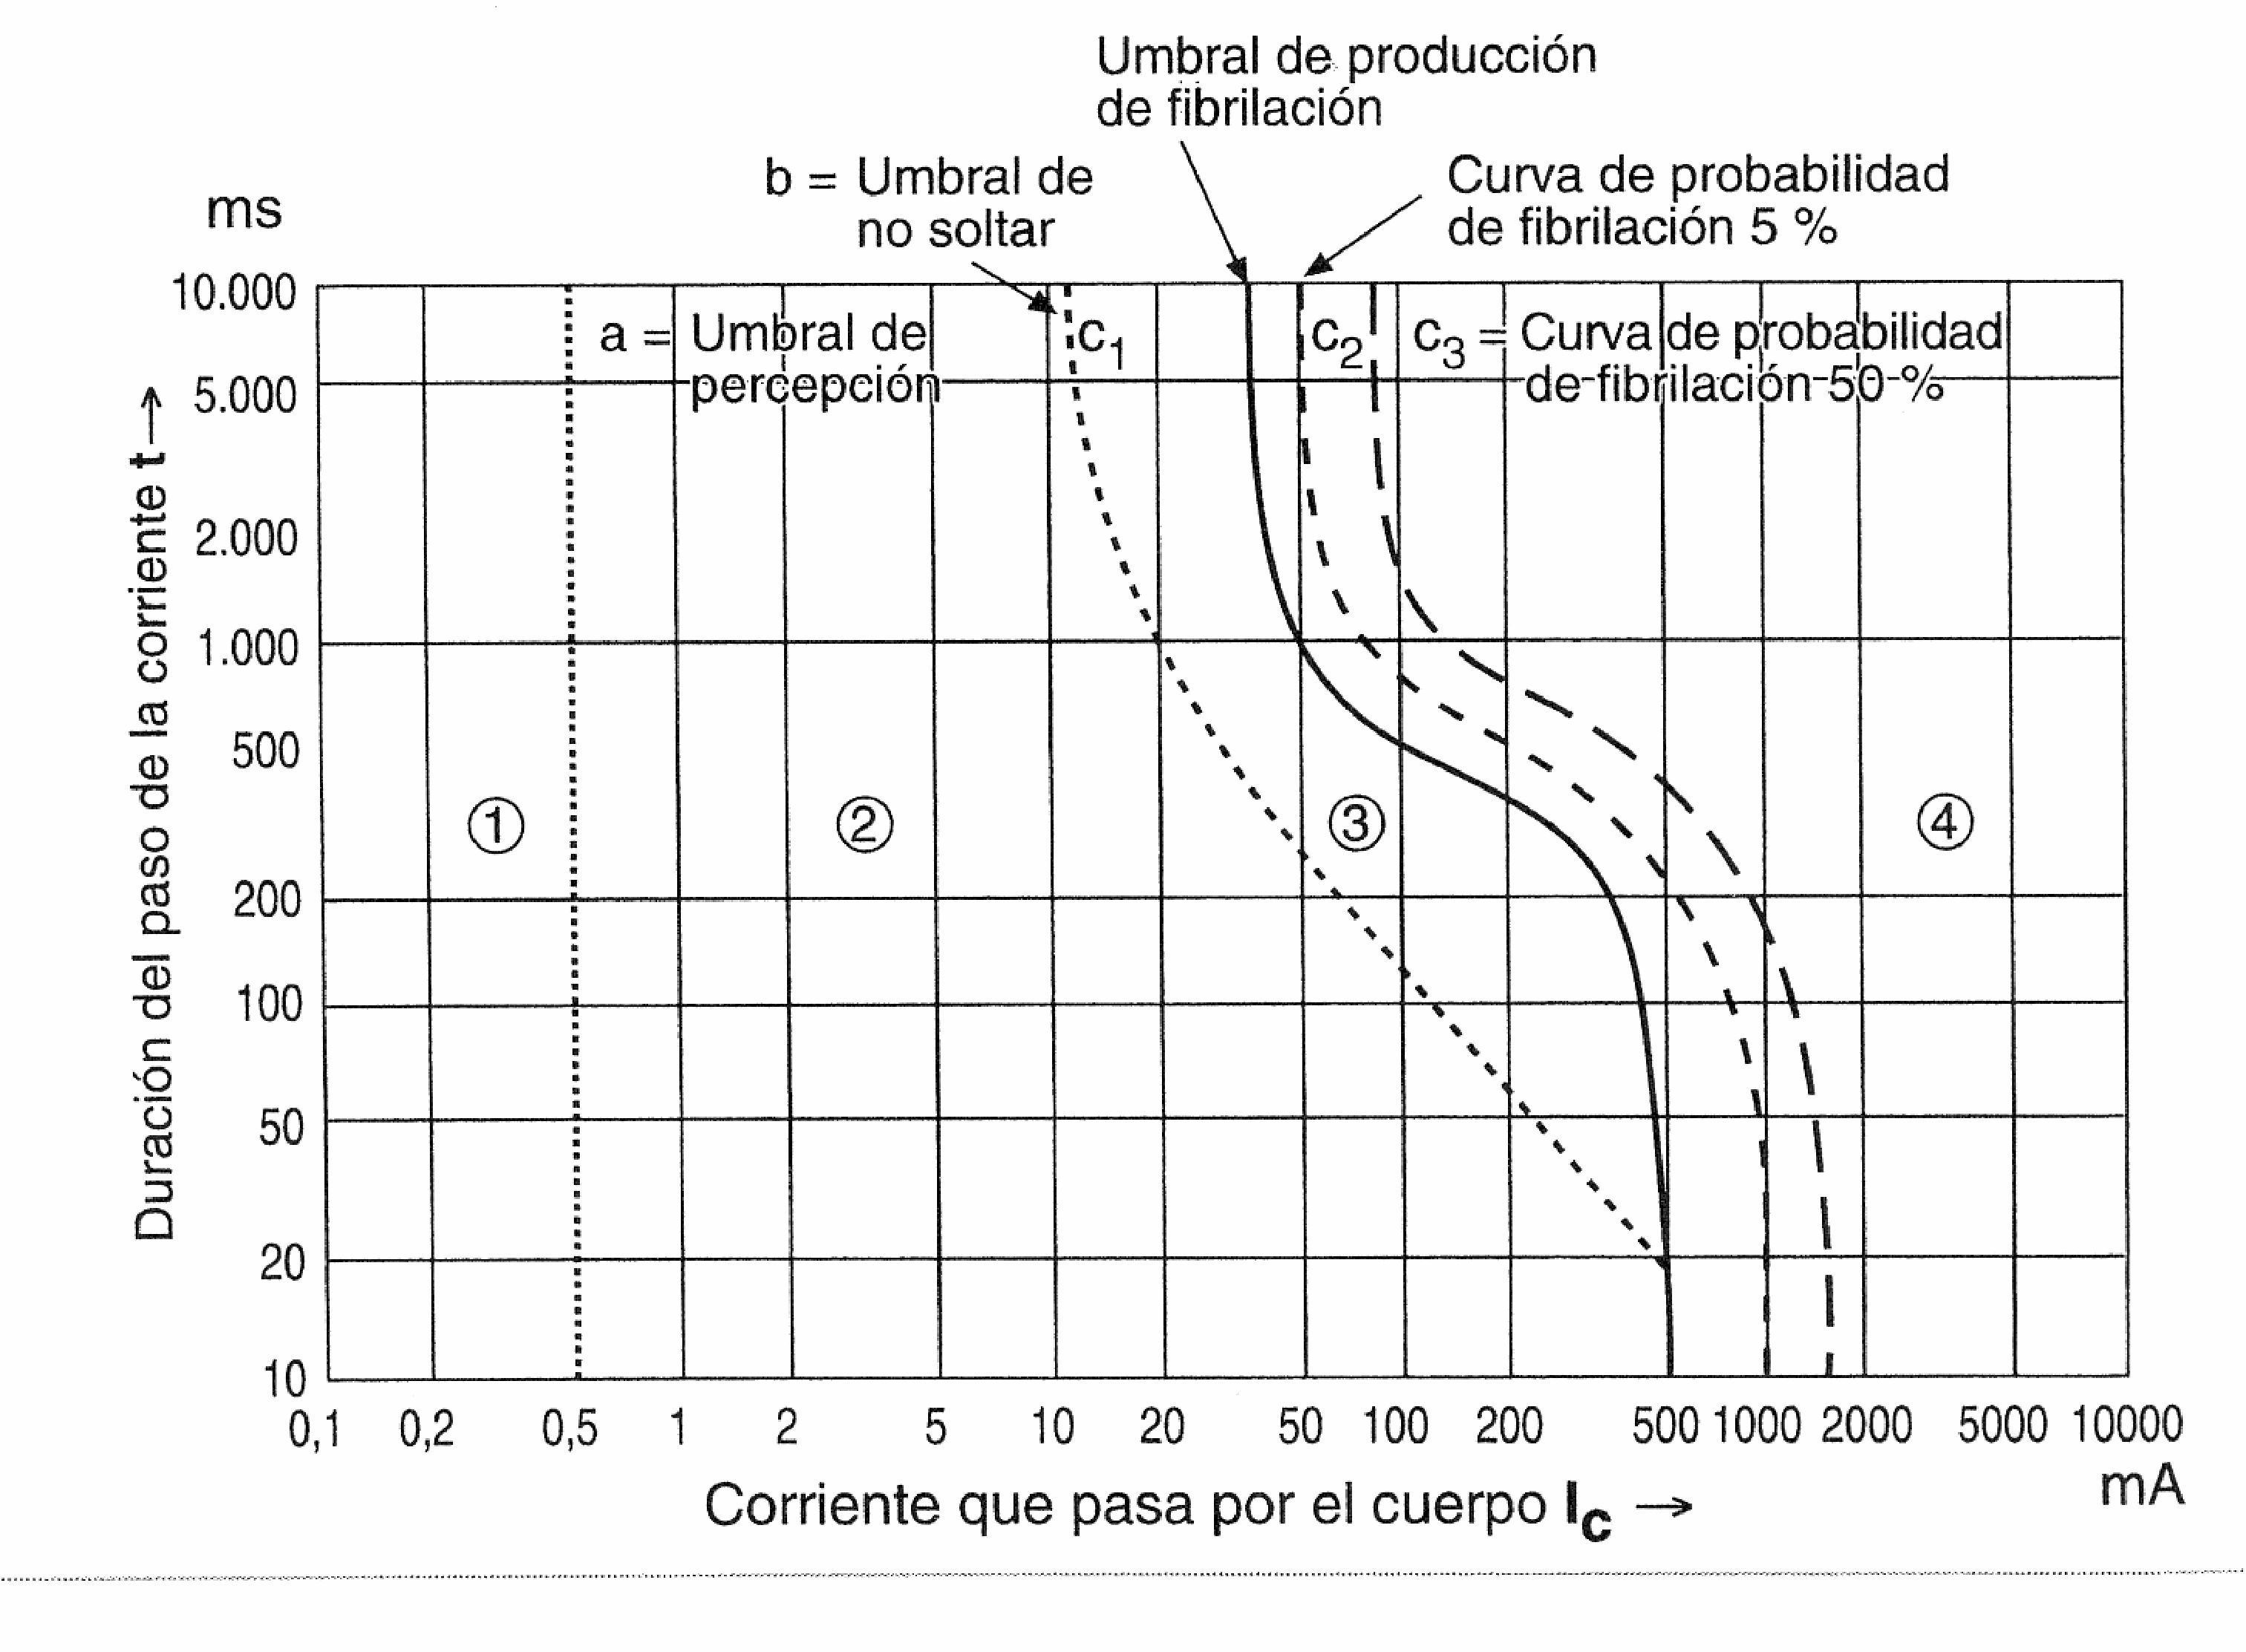
\includegraphics[scale=0.23]{../figs/CurvaIntensidadContactoTiempo}

\caption[Efecto de la corriente que circula por el cuerpo humano]{Efecto de la corriente que circula por el cuerpo humano según su
intensidad y tiempo de duración \cite{PerezGabarda2000,PerezGabarda2000a}.\label{fig:EfectoCorriente}}

\end{figure}


La intensidad que puede circular por el cuerpo depende de la tensión
de contacto y la resistencia expuesta. Por tanto, las medidas de seguridad
básicas consisten en reducir la tensión a la que se puede exponer
un ser humano y aumentar su resistencia (mediante el uso de guantes,
calzado, o aislamiento del suelo). 

La resistencia depende del estado de la piel, sudoración, estado físico,
superficie de contacto, presión. No es homogénea, siendo que cada
parte del cuerpo presenta valores diferentes. Tampoco es estable con
el tiempo sino que depende de la duración del contacto y de la tensión
aplicada: la resistencia disminuye con la tensión, realimentandose
los efectos de altos valores de tensión y baja resistencia. 

También la frecuencia eléctrica es un factor a tener en cuenta. Así,
la corriente continua es menos peligrosa que la alterna convencional,
pero puede producir electrolisis de la sangre. El umbral de percepción
se sitúa en $\SI{2}{\milli\ampere}$ y el umbral de control muscular
en $\SI{75}{\milli\ampere}$. La alterna convencional ($\SI{50}{\hertz}$)
tiene su umbral de percepción en $\SI{0.5}{\milli\ampere}$ y el umbral
de control muscular en $\SI{15}{\milli\ampere}$. Finalmente la corriente
alterna empleada en algunas aplicaciones industriales ($\SI{10}{\kilo\hertz}$)
presenta efectos más leves que la alterna convencional debido al efecto
pelicular%
\footnote{Según este efecto, la corriente tiende a circular por la piel con
frecuencias elevadas.%
}. Su umbral de percepción está en $\SI{5}{\milli\ampere}$ y el umbral
de control muscular en $\SI{75}{\milli\ampere}$.

Los efectos que produce la corriente dependen también de la trayectoria
que sigue al atravesar el cuerpo, siendo más graves cuando en el camino
se encuentran órganos vitales. Dado que esta trayectoria se realiza
siguiendo la ruta más corta o la de menor resistencia, la posibilidad
de atravesar órganos vitales dependerá de los puntos de contacto con
la tensión eléctrica. Los efectos también dependen de la edad, el
sexo, el estado físico, la fatiga o el miedo. 

En base a estas consideraciones, se establecen unos requisitos para
la tensión y la corriente de seguridad \cite{RD_842_2002,Gomez-Vidal2000,MestreRovira2002,PerezGabarda2000}: 
\begin{itemize}
\item Se establecen dos condiciones: emplazamientos secos o húmedos (instalaciones
de interior); emplazamientos mojados (instalaciones en intemperie).
\item Se define como tensión de seguridad la tensión de contacto máxima
admisible durante al menos cinco segundos. Para emplazamientos secos
es de $\SI{120}{\volt}$ para corriente continua y $\SI{50}{\volt}$
para corriente alterna. Para emplazamientos mojados es de $\SI{60}{\volt}$
para corriente continua y $\SI{24}{\volt}$ para corriente alterna.
\item La corriente máxima admisible se fija en $\SI{30}{\milli\ampere}$
para alterna y $\SI{100}{\milli\ampere}$ para continua.
\end{itemize}

\subsection{Protección contra contactos directos}

La figura \ref{fig:ContactoDirectoTT_TN} muestra los esquemas eléctricos
equivalentes a un contacto directo que se produce en un sistema fotovoltaico
cuando el esquema de conexión a tierra es TT o TN. En estos esquemas
el cuerpo humano está simbolizado por las resistencias $R_{h}$\nomenclature[Rh]{$R_{h}$}{Resistencia eléctrica equivalente de un ser humano}
(resistencia del cuerpo) y $R_{p}$\nomenclature[Rp]{$R_{p}$}{Resistencia eléctrica equivalente del contacto del cuerpo con el terreno}
(resistencia equivalente del contacto del cuerpo con el terreno).
$R_{ts}$\nomenclature[Rts]{$R_{ts}$}{Resistencia de la toma a tierra de servicio}
es la resistencia de la toma a tierra de servicio, que conecta un
conductor con la puesta a tierra, y $R_{tp}$\nomenclature[Rtp]{$R_{tp}$}{Resistencia de la toma a tierra de protección}
es la resistencia de la toma a tierra de protección, que conecta las
masas con la puesta a tierra en un esquema TT. En algunos casos, en
los esquemas TN es recomendable insertar una resistencia entre las
masas y la resistencia de servicio para aumentar la protección de
los equipos. Por simplicidad esta resistencia no ha sido incluida
aquí, aunque sí en la figura \ref{fig:ContactoIndirectoTN}.

%
\begin{figure}
\hfill{}\subfloat[Esquema TT.]{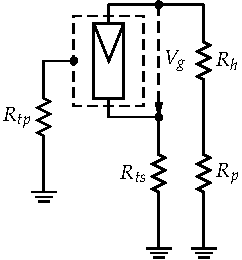
\includegraphics{../figs/ContactoDirectoTT}



}\hfill{}\subfloat[Esquema TN.]{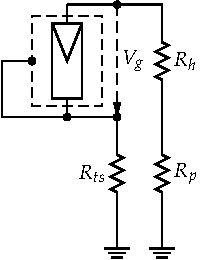
\includegraphics{../figs/ContactoDirectoTN}

}\hfill{}\subfloat[Esquema simplificado TT y TN.]{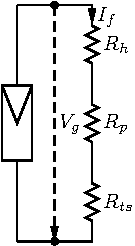
\includegraphics{../figs/ContactoDirectoTT_simple}

}\hfill{}

\caption{\label{fig:ContactoDirectoTT_TN}Esquema eléctrico de un contacto
directo en un sistema fotovoltaico con esquema de puesta a tierra
TT o TN.}

\end{figure}


En estas condiciones, la corriente que circula por el cuerpo depende
del valor de estas resistencias y de la tensión entregada por el generador.
El caso peor se produce cuando el generador se encuentra en circuito
abierto, $V_{ocG}$. Por tanto, la máxima corriente de fuga que puede
producirse, $I_{F,max}$\nomenclature[Ifmax]{$I_{F,max}$}{Corriente máxima de fuga admisible}\nomenclature[If]{$I_{F}$}{Corriente de fuga},
es:

\begin{equation}
I_{F,max}=\frac{V_{ocG}}{R_{h}+R_{p}+R_{ts}}\label{eq:IfmaxTT}\end{equation}


Cuando el esquema de conexión a tierra es IT, el contacto directo
no puede cerrar el circuito y por tanto $I_{F,max}=0$. Sin embargo,
es necesario tener en cuenta que la resistencia de aislamiento de
los equipos, y particularmente la de los módulos fotovoltaicos es
finita. Más aún, al conectar eléctricamente un número $N_{T}$\nomenclature[Nt]{$N_{T}$}{Número total de módulos en un generador}
de módulos, la resistencia de aislamiento del conjunto, $R_{iso}$\nomenclature[Riso]{$R_{iso}$}{Resistencia de aislamiento de un generador}\nomenclature[Risom]{$R_{iso}^{(m)}$}{Resistencia de aislamiento de un modulo},
es la equivalente al paralelo de las individuales, $R_{iso}^{(m)}$.
Es importante resaltar que $N_{T}$ es el número total de módulos
que componen el generador dado que la conexión de las resistencias
de aislamiento es en paralelo, independientemente de la configuración
eléctrica del generador (figura \ref{fig:RisoDistribuidaIT}). 

%
\begin{figure}
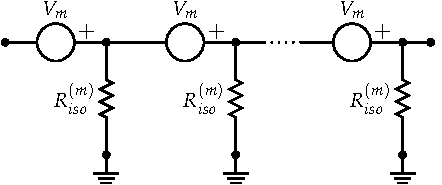
\includegraphics{../figs/ContactoDirectoIT}

\caption{\label{fig:RisoDistribuidaIT}Resistencia de aislamiento distribuida
en un generador fotovoltaico con esquema de conexión a tierra IT.}

\end{figure}


Así, la resistencia de aislamiento del generador, $R_{iso}$, es:\begin{eqnarray}
R_{iso} & = & \frac{R_{iso}^{(m)}}{N_{T}}\label{eq:RisoIT}\end{eqnarray}
y por tanto, se puede demostrar que la corriente de fuga máxima en
una conexión IT es \cite{Gomez-Vidal2000}: 

\begin{equation}
I_{f}=\frac{V_{ocG}}{R_{iso}+R_{h}}\label{eq:If_IT}\end{equation}


Siendo un sistema de corriente continua, la máxima corriente admisible
es inferior a $\SI{100}{\milli\ampere}$. Con este valor se puede
calcular la mínima resistencia de aislamiento que elimina el riesgo
por contactos directos:

\begin{equation}
I_{f}\leq100\, mA\Longrightarrow R_{iso}\geq10\cdot V_{ocG}-R_{h}\label{eq:Riso_IT}\end{equation}


Este análisis corresponde al funcionamiento en régimen permanente.
Si se tiene en consideración el transitorio debido a la capacidad
distribuida existente entre el generador y tierra (Figura \ref{fig:CapacidadIT})
se puede calcular la corriente de descarga que se producirá a través
del cuerpo humano procedente de esta capacidad. 

%
\begin{figure}
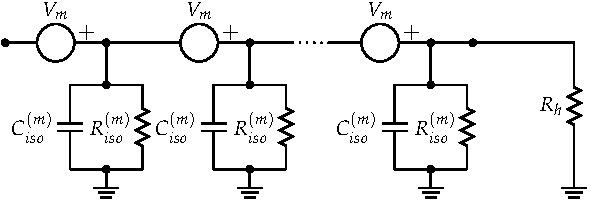
\includegraphics{../figs/ContactoDirectoIT_Capacidad}

\caption{Capacidad distribuida en un generador fotovoltaico con esquema de
conexión a tierra IT.\label{fig:CapacidadIT}}

\end{figure}


Salvo en sistemas defectuosos, se cumple $R_{iso}\gg R_{h}$ y por
tanto la asociación paralelo de la resistencia de aislamiento con la de la
persona puede aproximarse por esta última, $R_{iso}||R_{h} \simeq R_h$. El comportamiento
eléctrico de un ser humano puede ser representado con una resistencia
tipo de $R_{h}=\SI{1000}{\ohm}$. Para la capacidad es posible adoptar
un valor de $C_{iso}=\SI{1}{\micro\farad}$\nomenclature[Ciso]{$C_{iso}$}{Capacidad distribuida de un generador fotovoltaico con esquema de conexión a tierra IT}
de acuerdo a ensayos en sistemas reales \cite{Gomez-Vidal2000}.
De esta forma, la constante de tiempo de este sistema es $T\simeq C_{iso}\cdot R_{h}=\SI{1}{\milli\second}$.
Según la norma CEI479-2 la corriente de descarga tiene una duración
equivalente a tres veces la constante de tiempo del circuito, $T_{desc}=3\cdot T=\SI{3}{\milli\second}$
y se calcula con:

\begin{eqnarray}
I_{desc} & = & \frac{V_{ocG}}{R_{h}\cdot\sqrt{6}}\label{eq:IdescIT}\end{eqnarray}
\nomenclature[Idesc]{$I_{desc}$}{Corriente de descarga de la capacidad distribuida en un generador fotovoltaico con esquema de conexión a tierra IT}

Según la norma CEI479-2, dado que la descarga dura $\SI{3}{\milli\second}$,
se necesitan tensiones de generador superiores a los $\SI{1000}{\volt}$
para producir dolor, y tensiones superiores a los $\SI{3000}{\volt}$
para que exista riesgo por fibrilación \cite{PerezGabarda2000a}.


\subsection{Protección contra contactos indirectos}

En un contacto indirecto la persona toma contacto con una parte del
sistema que no debiera estar puesta a potencial (por ejemplo, la estructura
metálica, el marco de los módulos o las carcasas de los equipos eléctricos).
Sin embargo, algún defecto del sistema puede provocar que la resistencia
de aislamiento sea demasiado baja, produciéndose un camino por el
que fluye la corriente de fuga, exponiendo a la persona a un potencial
de contacto peligroso. En las figuras que se muestran a continuación
se supone que el contacto se produce en el marco del generador fotovoltaico,
representado con una línea discontinua.

Cuando el esquema de conexión a tierra es TT, un contacto indirecto
como el representado en la figura \ref{fig:ContactoIndirectoTT} produce
una tensión de contacto, $V_{c}$\nomenclature[Vc]{$ V_{c}$}{Tensión de contacto},
que depende de la corriente de fuga y la resistencia de la tierra
de protección. Es posible demostrar que la máxima corriente de fuga
posible es la de cortocircuito del generador \cite{Gomez-Vidal2000}.
Por tanto, 

\begin{equation}
V_{c}\simeq I_{scG}\cdot R_{tp}\label{eq:VcIndirectoTT}\end{equation}


%
\begin{figure}
\hfill{}\subfloat[]{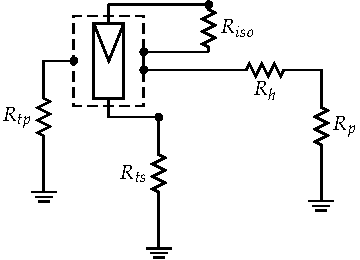
\includegraphics{../figs/ContactoIndirectoTT}

}\hfill{}\subfloat[]{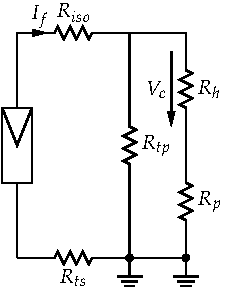
\includegraphics{../figs/ContactoIndirectoTT_simple}

}\hfill{}

\caption{Esquema eléctrico de contacto indirecto en un sistema fotovoltaico
con esquema de conexión a tierra TT.\label{fig:ContactoIndirectoTT}}

\end{figure}


Cuando el esquema de conexión a tierra es TN (figura \ref{fig:ContactoIndirectoTN})
el circuito se cierra a través de la resistencia de aislamiento del
generador y de la resistencia $R$ que conecta la toma a tierra con
el conductor puesto a tierra. Por tanto, el contacto indirecto no
produce tensión en el ser humano, $V_{c}=0$, aunque sí existirá una
corriente de fuga cuyo valor depende de la resistencia de aislamiento
del generador y de la resistencia $R$ (ecuación \ref{eq:IfugaTN}):

%
\begin{figure}
\hfill{}\subfloat[]{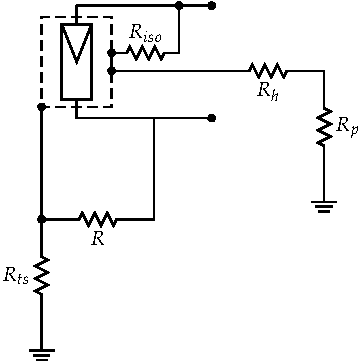
\includegraphics{../figs/ContactoIndirectoTN}

}\hfill{}\subfloat[]{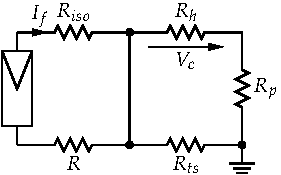
\includegraphics{../figs/ContactoIndirectoTN_simple}

}\hfill{}

\caption{Esquema eléctrico de contacto indirecto en un sistema fotovoltaico
con esquema de conexión a tierra TN.\label{fig:ContactoIndirectoTN}}

\end{figure}


\begin{equation}
I_{F,max}=\frac{V_{ocG}}{R_{iso}+R}\label{eq:IfugaTN}\end{equation}


Cuando el esquema de conexión a tierra es IT, un contacto indirecto
como el representado en la figura \ref{fig:ContactoIndirectoIT} no
puede cerrar el circuito. En esta situación no existirá corriente
de fuga, $I_{F}=0$, y la persona no estará expuesta a tensión de
contacto, $V_{c}=0$.

%
\begin{figure}
\hfill{}\subfloat[]{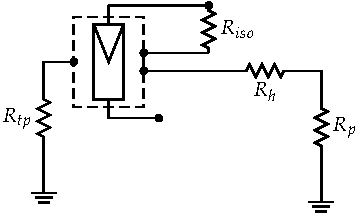
\includegraphics{../figs/ContactoIndirectoIT}

}\hfill{}\subfloat[]{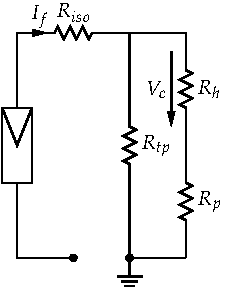
\includegraphics{../figs/ContactoIndirectoIT_simple}

}\hfill{}

\caption{Esquema eléctrico de contacto indirecto en un sistema fotovoltaico
con esquema de conexión a tierra IT.\label{fig:ContactoIndirectoIT}}

\end{figure}



\subsection{Resumen de protecciones}

Según la ITC-BT-24 las protecciones a utilizar para proteger frente
a contactos directos deben estar basadas en evitar que una persona
pueda entrar en contacto con las partes activas de la instalación,
e incluye una protección complementaria cuando las anteriores no consiguen
su objetivo:
\begin{itemize}
\item Protección por aislamiento de las partes activas.
\item Protección por medio de barreras o envolventes.
\item Protección por medio de obstáculos.
\item Protección por puesta fuera de alcance por alejamiento.
\item Protección complementaria por dispositivos de corriente diferencial-residual.
\end{itemize}
Esta misma ITC-BT-24 recoge las formas de protección para contactos
indirectos:
\begin{itemize}
\item Protección por corte automático de la alimentación: cuando se produce
el contacto, el objetivo es evitar que la fuente eléctrica siga alimentando
la fuga.
\item Protección por empleo de equipos de clase II%
\footnote{Véase la definición aportada al principio de este capítulo.%
} o por aislamiento equivalente, con la misión de alcanzar resistencias
de aislamiento de alto valor y estables en el tiempo.
\item Puesta a tierra, como camino preferente para conducir la corriente
de fuga y para servir de potencial común para todos los elementos
que entran en contacto con ella.
\end{itemize}
En un sistema fotovoltaico es de uso común que el esquema de tierra
sea IT en la zona del generador fotovoltaico y TT a partir de la salida
del inversor. En este contexto, todo el sistema de protecciones reseñado
se puede condensar en tres niveles \cite{Gomez-Vidal2000}:
\begin{itemize}
\item Nivel 1: Refuerzo del aislamiento de las partes activas. 
\item Nivel 2: Sistema de detección de aislamiento.
\item Nivel 3: Puesta a tierra.
\end{itemize}
El nivel 1, o refuerzo del aislamiento de las partes activas incluye
las siguientes medidas:
\begin{itemize}
\item Configuración flotante del generador: se impiden los accidentes por
contactos indirectos. 
\item Cableado con aislamiento de protección para reforzar la protección
contra contactos indirectos%
\footnote{Se suele aceptar que un módulo fotovoltaico está dotado de las características
propias de un material de clase II. La combinación de módulos fotovoltaicos
con cableado con aislamiento de protección cumple así el requerimiento
de emplear materiales de clase II exigido por la ITC-BT-24 para evitar
contactos indirectos.%
}. 
\item Aislamiento galvánico AC-DC: Mediante transformadores de devanados
independientes en los inversores se imposibilita el cierre de corriente
de fallo a través del inversor.
\end{itemize}
El nivel 2, o sistema de detección de aislamiento abarca las medidas
necesarias para comprobar el adecuado funcionamiento del nivel 1 y
las actuaciones a llevar a cabo cuando el nivel 1 ha fallado. Para
la vigilancia es común el empleo de un vigilante de aislamiento. Una
posible implementación consiste en un equipo que genera una señal
de baja frecuencia (2 a 5 Hz) para evitar las fugas capacitivas del
cableado, la inyecta en un polo activo y mide la corriente de retorno
por tierra, obteniendo así una medida indirecta de la resistencia
de aislamiento. Cuando el valor obtenido se encuentra por debajo de
cierto umbral (característico del sistema, tal y como describe la
ecuación \ref{eq:RisoIT}) el vigilante ordena una secuencia de acciones
para evitar el accidente eléctrico. La secuencia más recomendable
debe comprender la parada y desconexión del inversor, el cortocircuito
del generador fotovoltaico y la puesta a tierra del mismo. Sin embargo,
esta secuencia conlleva la utilización de varios elementos de protección
que pueden encarecer en demasía el equipo inversor. Por esta razón,
algunos equipos de menor potencia optan por desconectar al inversor
del generador (a pesar de que en esta situación la tensión del campo
fotovoltaico es la máxima disponible) y otros optan por continuar
funcionando pero activan una alarma que puede ser visual o comunicada
telemáticamente.

Los dos niveles anteriores se asientan sobre el nivel 3, que proporciona
la protección de la puesta a tierra directa de todas las masas accesibles
de la planta. Gracias a ella se consigue limitar la tensión que con
respecto a tierra puedan adquirir las masas en caso de derivación,
y se dota de un potencial común a todas las masas accesibles de forma
simultánea%
\footnote{Cuando dos masas pertenecientes a dos equipos diferentes son accesibles
simultáneamente por una única persona, es posible que, ante un defecto
de funcionamiento, entre las dos masas aparezca una tensión peligrosa
para un ser humano. La equipotencialidad de una toma a tierra común
evita la aparición de estas tensiones.%
}.


\subsection{Puesta a tierra}
\label{sec:puesta_tierra}
Un sistema de puesta a tierra consta de la toma a tierra (generalmente
picas o placas metálicas resistentes a la corrosión), un conjunto
de conductores de tierra que conectan la toma a tierra con el borne
principal de tierra, lugar al que van conectados los conductores de
unión equipotencial (para mantener el mismo potencial con otros elementos
parcialmente enterrados, como canalizaciones metálicas) y los conductores
de protección, que unen las masas con la toma a tierra. Es importante
remarcar la necesidad de que todos los elementos del sistema de puesta
a tierra de un sistema fotovoltaico estén interconectados. De esta
forma, todas las masas metálicas accesibles por una persona están
conectadas a una superficie equipotencial, disminuyendo así la posibilidad
de aparición de tensiones peligrosas entre masas que pertenecen a
equipos diferentes.

Para el cálculo de la resistencia de la puesta a tierra constituida
por una única pica vertical, es aplicable la ecuación $R_{t}=\frac{\rho}{L_{p}}$\nomenclature[Rt]{$R_{t}$}{Resistencia de la puesta a tierra}\nomenclature[rho_t]{$\rho$}{Resistividad del terreno},
siendo $\rho$ la resistividad del terreno y $L_{p}$\nomenclature[Lpica]{$L_{p}$}{Longitud de una pica de puesta a tierra}
la longitud de la pica. De forma orientativa, la tabla \ref{tab:ValoresResistividad}
ofrece unos valores medios aproximados de resistividad en función
del terreno.

%
\begin{table}
\caption{Valores medios aproximados de la resistividad en función del terreno
según la ITC-BT-18.\label{tab:ValoresResistividad}}


\begin{tabular}{lr}
\toprule 
Terrenos cultivables fértiles & $\SI{50}{\ohm\meter}$\tabularnewline
\midrule 
Terrenos cultivables poco fértiles & $\SI{500}{\ohm\meter}$\tabularnewline
\midrule 
Suelos pedregosos & $\SI{3000}{\ohm\meter}$\tabularnewline
\bottomrule
\end{tabular}
\end{table}


Para mejorar la resistencia de la puesta a tierra, se utilizan varios
electrodos interconectados separados una cierta distancia. En términos
generales, es suficiente con ubicar una pica cada $\SI{10}{\meter}$
o $\SI{15}{\meter}$. La resistencia equivalente del conjunto puede
aproximarse por el paralelo de las individuales. Así, denotando con
$n_{p}$\nomenclature[np]{$n_{p}$}{Número de picas interconectadas en una puesta a tierra}
el número de picas que componen el sistema de puesta a tierra, su
resistencia es:
\begin{equation}
R_{t} \simeq \frac{\rho}{n_{p}\cdot L_{p}}
\label{eq:Rtvariaspicas}
\end{equation}


Por ejemplo, para conseguir una $R_{t}=\SI{5}{\ohm}$ en un terreno
con $\rho=\SI{100}{\ohm}$ se deberán utilizar aproximadamente 10
picas de una longitud de 2 metros (cada una de ellas tendrá una resistencia
$R_{t,i}=\SI{50}{\ohm}$). 

Una de las misiones de la puesta a tierra consiste en disminuir la
tensión de contacto que aparece al circular una corriente de fugas
durante un contacto indirecto. Los esquemas IT y TN no producen tensión
de contacto en el primer contacto indirecto y, por tanto, sólo el
esquema TT necesita \emph{esta} función de la puesta a tierra. En
este esquema, suponiendo la existencia de un dispositivo de protección
(por ejemplo, un vigilante de aislamiento) que limita la corriente
de fuga, el valor de la resistencia de la puesta a tierra debe cumplir:

\begin{equation}
R_{tp}\leq\frac{V_{max}}{I_{f}}\label{eq:Rtp_TT}\end{equation}


Apliquemos la ecuación \ref{eq:Rtp_TT} a un ejemplo concreto. Una
instalación fotovoltaica se considera local mojado%
\footnote{Según la ITC-BT-30, se consideran como locales o emplazamientos mojados
las instalaciones a la intemperie.%
}, así que la máxima tensión de contacto admisible en la zona de corriente
continua es $V_{max}=\SI{60}{\volt}$. Al ser corriente continua la
máxima corriente admisible que puede circular por el cuerpo humano
es $I_{max}=\SI{100}{\milli\ampere}$. Si este generador fotovoltaico
utiliza el esquema TT e incorpora un dispositivo de protección que
limite la corriente de fuga, deberá emplear una toma a tierra que
cumpla $R_{tp}\leq\SI{600}{\ohm}$.

Un esquema IT es intrínsecamente seguro ante contactos indirectos,
pero es posible que el generador fotovoltaico ya haya tenido un primer
defecto a tierra. Si permaneciendo este primer fallo se produce un
contacto indirecto adicional, el sistema produce una tensión de contacto
que hay que limitar. En esta situación, dado que el primer fallo a
tierra transforma el esquema IT en un esquema TT, el valor límite
de la resistencia de la puesta a tierra en ausencia de un dispositivo
que limite la corriente de fuga es:

\begin{equation}
R_{tp}\leq\frac{V_{max}}{I_{sc}}\label{eq:Rtp_IT2}\end{equation}
\nomenclature[Vmax]{$V_{max}$}{Tensión máxima admisible de seguridad ante un contacto}

Consideremos ahora la instalación fotovoltaica anterior con un esquema
IT. Suponiendo que el generador tiene una corriente de cortocircuito
igual a $I_{sc}=\SI{150}{\ampere}$, para proteger frente a la eventualidad
de la combinación de un primer fallo a tierra con un segundo contacto
indirecto, suponiendo que el sistema no incorpora un dispositivo que
limite la corriente de fuga (o para proteger también frente a la posibilidad
de que éste no realice correctamente su función) la resistencia de
la puesta a tierra debe ser ahora $R_{tp}\leq\SI{0.4}{\ohm}$.

Este segundo cálculo arroja un valor difícilmente alcanzable en un
terreno con valores de resistividad eléctrica normales dentro de ciertos
costes razonables. En general, se suele adoptar como requisito mínimo
el resultado de la ecuación \ref{eq:Rtp_TT} aplicado a la zona de
corriente alterna (por tanto, empleando $V_{max}=\SI{24}{\volt}$
y $I_{max}=\SI{30}{\milli\ampere}$). Con este primer resultado se
diseña un sistema de puesta a tierra. Según las condiciones del terreno,
la accesibilidad a personas y coste asumible, se intenta mejorar la
puesta a tierra con la vista puesta en el resultado de la ecuación
\ref{eq:Rtp_IT2} aplicada al generador fotovoltaico.

A la hora de realizar puestas a tierra en lugares donde ya existen
tomas a tierra que pertenecen a otras instalaciones eléctricas es
importante entender su funcionalidad para tomar la decisión correcta.
Cuando el sistema de tierra existente corresponda a la instalación
de Baja Tensión del edificio en el que se ubicará el SFCR (situación
habitual en la integración en edificios), se utilizará la puesta a
tierra existente para conectar las masas del sistema fotovoltaico.
De esta forma, todas las masas metálicas accesibles para una persona
estarán unidas a una superficie equipotencial y así, en caso de fallo
de aislamiento, no podrá estar expuesto a una tensión peligrosa. Cuando
el sistema de tierras existente corresponde al neutro de Media Tensión
del transformador de la compañía eléctrica es necesario separarse
suficientemente para no interferir en su funcionamiento%
\footnote{Por ejemplo, el artículo 12 del RD1663/2000 dice expresamente que
{}``la puesta a tierra de las instalaciones fotovoltaicas interconectadas
se hará siempre de forma que no se alteren las condiciones de puesta
a tierra de la red de la empresa distribuidora''.%
}. Según la ITC-BT-08, dos tomas de tierra son independientes cuando
al circular la máxima corriente de defecto por una de ellas, la otra
no alcance, respecto a un punto de potencial cero, una tensión superior
a $\SI{50}{\volt}$. Para terrenos de resistividad no elevada ($\rho<\SI{100}{\ohm\meter}$),
esta condición se cumple para distancias superiores a $\SI{15}{\meter}$.


\section{Protección de los equipos}


\subsection{Tormentas eléctricas}

En el interior de las nubes se producen corrientes de aire con suficiente
velocidad como para atomizar las partículas de agua y hielo del interior
y dotarlas de carga electrostática. Las partículas cargadas positivamente
ascienden a las capas superiores de las nubes y las negativas permanecen
en la base (figura \ref{fig:Formaci=0000F3nRayo}). Esta separación
de cargas produce un campo eléctrico en el interior del núcleo tormentoso.
Por otra parte, las cargas negativas de las capas inferiores atraen
a las cargas positivas de la superficie terrestre. Cuando el campo
eléctrico interno de la nube alcanza la ruptura del aire, se producen
las descargas eléctricas hacia la superficie terrestre. Esta descarga
comienza en la nube con un trazador descendente. Cuando este trazador
se acerca a una distancia de entre 10 a 100 m de la tierra, se generan
diversos trazadores ascendentes desde la superficie terrestre en busca
del trazador descendente. Aquel trazador ascendente que conecta con
el descendente cierra la descarga y determina el lugar del impacto.

%
\begin{figure}
\begin{centering}
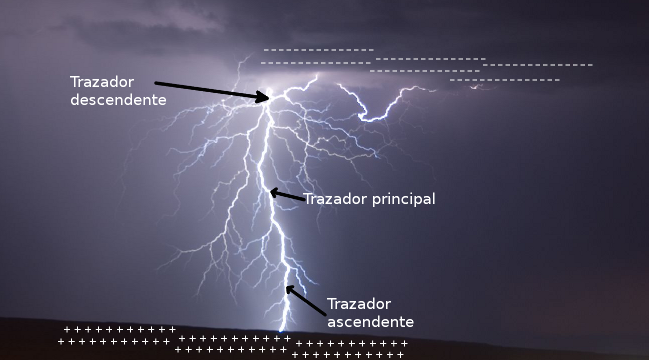
\includegraphics[scale=0.65]{../figs/Tormenta}
\end{centering}

\caption[Formación de un rayo eléctrico.]{\label{fig:Formaci=0000F3nRayo}Formación de un rayo eléctrico {\footnotesize (imagen
elaborada a partir de la fotografía disponible en }\protect \\
{\footnotesize \protect\url{http://commons.wikimedia.org/wiki/File:DC16_Lightning.jpg})}. }

\end{figure}


La descarga está determinada principalmente por el campo eléctrico
interno de la nube. Sólo cuando el trazador se encuentra a una distancia
de entre 10 a 100 metros, las condiciones locales suponen una influencia
determinante en la localización del impacto. Por ejemplo, las construcciones
metálicas de mayor altura (antenas) o superficie (instalaciones fotovoltaicas)
favorecen la formación de trazadores ascendentes que conecten con
el descendente. Por tanto, las instalaciones fotovoltaicas no aumentan
la probabilidad de descargas locales, pero una vez que se producen,
son lugares con mayor probabilidad de impacto.


\subsection{Sobretensión inducida}

El efecto de una descarga eléctrica sobre un sistema fotovoltaico
se manifiesta mayoritariamente en forma de sobretensión inducida.
Esta sobretensión aparece por tres fenómenos de acoplamiento diferenciados:
el galvánico, el capacitivo y el inductivo \cite{Becker.Vaaben.ea2000}.

El acoplamiento galvánico surge cuando la descarga se produce de forma
directa sobre alguna parte del sistema. En esta situación, los elementos
metálicos conducen la corriente de la descarga, pudiéndose producir
corrientes paralelas cuando el aislamiento de los cables o equipos
no es capaz de confinar la corriente en el conductor.

El acoplamiento capacitivo en el generador fotovoltaico se debe a
la existencia de cargas positivas en la superficie terrestre atraídas
por la carga negativa de la base del núcleo tormentoso. Este sistema,
cuya estructura está conectada eléctricamente a tierra, quedará cargado
positivamente. Cuando se produce la descarga eléctrica, la distribución
de cargas cambia súbitamente. Como un condensador que se descarga
de forma violenta, circulará una corriente de valor elevado y la tensión
respecto a tierra cambiará rápidamente. 

Para entender el acoplamiento inductivo hay que recordar que una descarga
eléctrica supone una corriente de gran valor en un lapso de tiempo
muy corto%
\footnote{El 50\% de las descargas conducen $\SI{30}{\kilo\ampere}$, con un
ratio de $\SI{20}{\kilo\ampere\per\micro\second}$ \cite{Becker.Vaaben.ea2000}.%
}, originando una inducción magnética a su alrededor. Según describe
la ley de Faraday-Lenz, un campo magnético variable produce una fuerza
electromotriz proporcional a la variación de su flujo. Así, aquellos
conductores que, a modo de antena, capten el flujo magnético derivado
de la descarga, desarrollarán una sobretensión inducida en sus extremos
(figura \ref{fig:InduccionGenerador}).

%
\begin{figure}
\begin{centering}
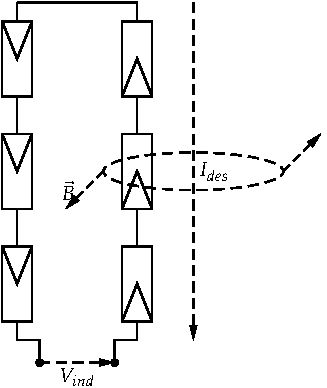
\includegraphics{../figs/SobretensionInducida}
\end{centering}

\caption{\label{fig:InduccionGenerador}Inducción sobre un generador.}

\end{figure}


El valor de la sobretensión depende de la velocidad del cambio del
flujo magnético. Asumiendo que el flujo magnético es proporcional
al campo magnético y al área que atraviesa, pueden distinguirse cuatro
factores que determinan la sobretensión inducida: tiempo de aparición
y extinción de la descarga, distancia de la descarga al generador,
intensidad de la descarga y área efectiva del generador. Los tres
primeros factores dependen del mecanismo formador de la tormenta,
ante los cuáles el diseñador y el instalador poco pueden hacer. Sin
embargo, el área efectiva que el generador fotovoltaico ofrece a la
inducción magnética son responsabilidad directa tanto del diseñador
como del instalador. Cuando el cableado del generador recorre el perímetro,
el bucle eléctrico tiene un área similar a la del generador. De esta
forma, al ocurrir una descarga eléctrica, el flujo magnético será
probablemente alto. Para reducir el flujo captado los conductores
deben ser guiados a lo largo de caminos cercanos, de forma que la
superficie de captación que forman sea la mínima necesaria. Además,
cada cierta distancia se deben realizar cruzamientos entre los cables
y así crear bucles anidados con signos alternos que contribuyen a
reducir aún más el flujo captado. Esta estrategia se emplea en ciertas
ocasiones en las redes de distribución eléctrica, tal y como se aprecia
en la figura \ref{fig:CruzamientoLineas}.

%
\begin{figure}


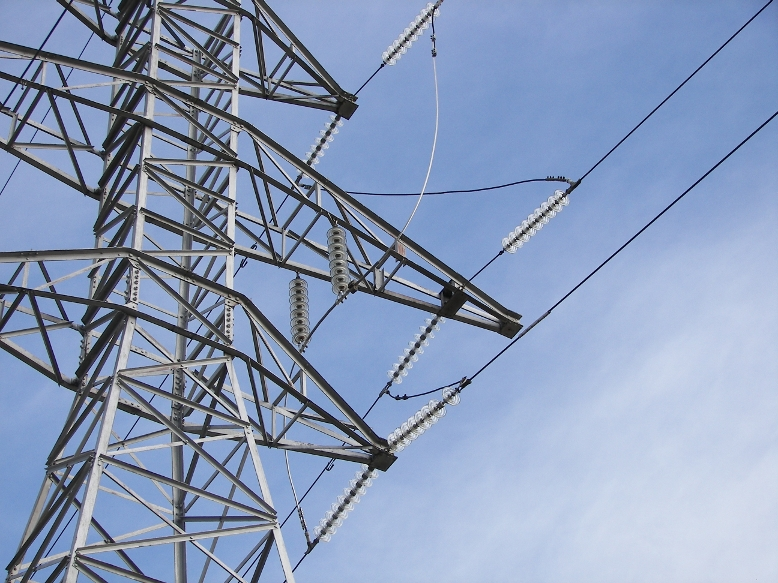
\includegraphics[scale=0.4]{../figs/CruzamientoLineaAerea}

\caption{Cruzamiento de líneas en una red aerea para aumentar la protección
contra sobretensiones.\label{fig:CruzamientoLineas}}



\end{figure}



\subsection{Sistemas de protección}

Los sistemas de protección se dividen en métodos de protección externa
frente a descargas y métodos de protección frente a sobretensiones.

Un sistema de protección externa frente a descarga tiene la tarea
de captar y conducir adecuadamente la descarga para evitar que impacte
sobre el objeto a proteger. Se compone de un terminal aéreo, el conductor
de bajada (que, en caso de ser varios, deberán estar interconectados)
y la red de puesta a tierra. El terminal aéreo capta la descarga y
la conduce a través del conductor de bajada hasta la red de tierra,
que deberá difundir la corriente de forma segura en la superficie.
Dado que este sistema de protección puede conducir impulsos de corriente
de alto valor, generará campos magnéticos a su alrededor, con el consiguiente
peligro de sobretensión. Es necesario respetar una distancia de seguridad
(más de $\SI{1}{\meter}$) entre los conductores de bajada y la instalaciones
metálicas cercanas. Si no se puede respetar esta distancia, el sistema
de puesta a tierra de la protección externa y la estructura metálica
deben interconectarse para evitar la aparición de arcos entre conductores
al circular la descarga. Por el contrario, si la distancia es superior
a la de seguridad, los sistemas de puesta a tierra deben ser independientes%
\footnote{Según la ITC-BT-08, dos tomas de tierra son independientes cuando
al circular la máxima corriente de defecto por una de ellas, la otra
no alcance, respecto a un punto de potencial cero, una tensión superior
a $\SI{50}{\volt}$.%
}.

La utilización de un sistema de protección externa depende de dos
factores principales: la probabilidad estadística de tormentas eléctricas
en la zona%
\footnote{El cálculo de esta probabilidad requiere del uso de mapas de nivel
isoceráunico y puede ser estimada mediante el procedimiento descrito
en el apartado 4.2 de \cite{Becker.Vaaben.ea2000}.%
} y el tamaño del sistema a proteger. En general, los sistemas fotovoltaicos
cuya potencia es inferior a $\SI{500}{\Wp}$ (por ejemplo, los
sistemas domésticos de electrificación rural) no requieren de sistemas
protección externa. 

Los métodos de protección frente a sobretensiones persiguen igualar
los diferentes potenciales que se producen en el momento en el que
se aparece la sobretensión a uno común de seguridad. Por tanto, estos
métodos están formados por una red de tierras que proporciona el potencial
común y por dispositivos que, cuando es necesario, conectan los conductores
a proteger a este potencial común. Los varistores suelen ser empleados
para cumplir esta función. El comportamiento de un varistor se asemeja
a una resistencia variable con la tensión, con un valor muy alto cuando
la tensión está por debajo de un umbral (de forma que todos los conductores
permanecen desconectados de tierra en funcionamiento normal) y con
valor casi nulo cuando se supera el umbral (de forma que todos los
conductores son conectados a tierra durante la breve duración de la
sobretensión). Estos dispositivos tienen un tiempo de actuación bajo
(inferior a los $\SI{25}{\nano\second}$) y una corriente máxima de
actuación de $\SI{15}{\kilo\ampere}$, con una tensión residual inferior
a $\SI{2}{\kilo\volt}$. 

Es importante tener en cuenta que cuando un varistor actúa, realiza
un cortocircuito entre sus conexiones. De ahí que se deba evitar su
ubicación entre elementos que puedan interactuar de forma dañina cuando
se produce un cortocircuito. Por ejemplo, la figura \ref{fig:EfectosVaristor}
muestra el estado en el que quedó una caja de protecciones después
de que los varistores que albergaba entrasen en funcionamiento. Esta
caja estaba conectada a la salida del generador fotovoltaico y de
ella partían varios metros de cable hasta el inversor DC/AC. Pero
los varistores no eran el último elemento de la caja: entre ellos
y la salida se instalaron sendos fusibles en cada polo. ¿Qué ocurrió?
Cuando los varistores entraron en funcionamiento para intentar reducir
una sobretensión atmosférica, se comportaron como un cortocircuito.
Este camino fácil ofrecido por los varistores fue aprovechado por
los condensadores que los inversores tienen en la entrada para descargar
su carga almacenada. Esta descarga adicional podía ser asumida sin
problemas por los varistores, pero también atravesó a los fusibles,
que no estaban capacitados para hacer frente a esta intensidad. Los
fusibles explotaron y con ellos todos los elementos de la caja. La
solución fue sencilla: se retiraron todos los fusibles situados entre
los varistores y el inversor.

%
\begin{figure}
\begin{centering}
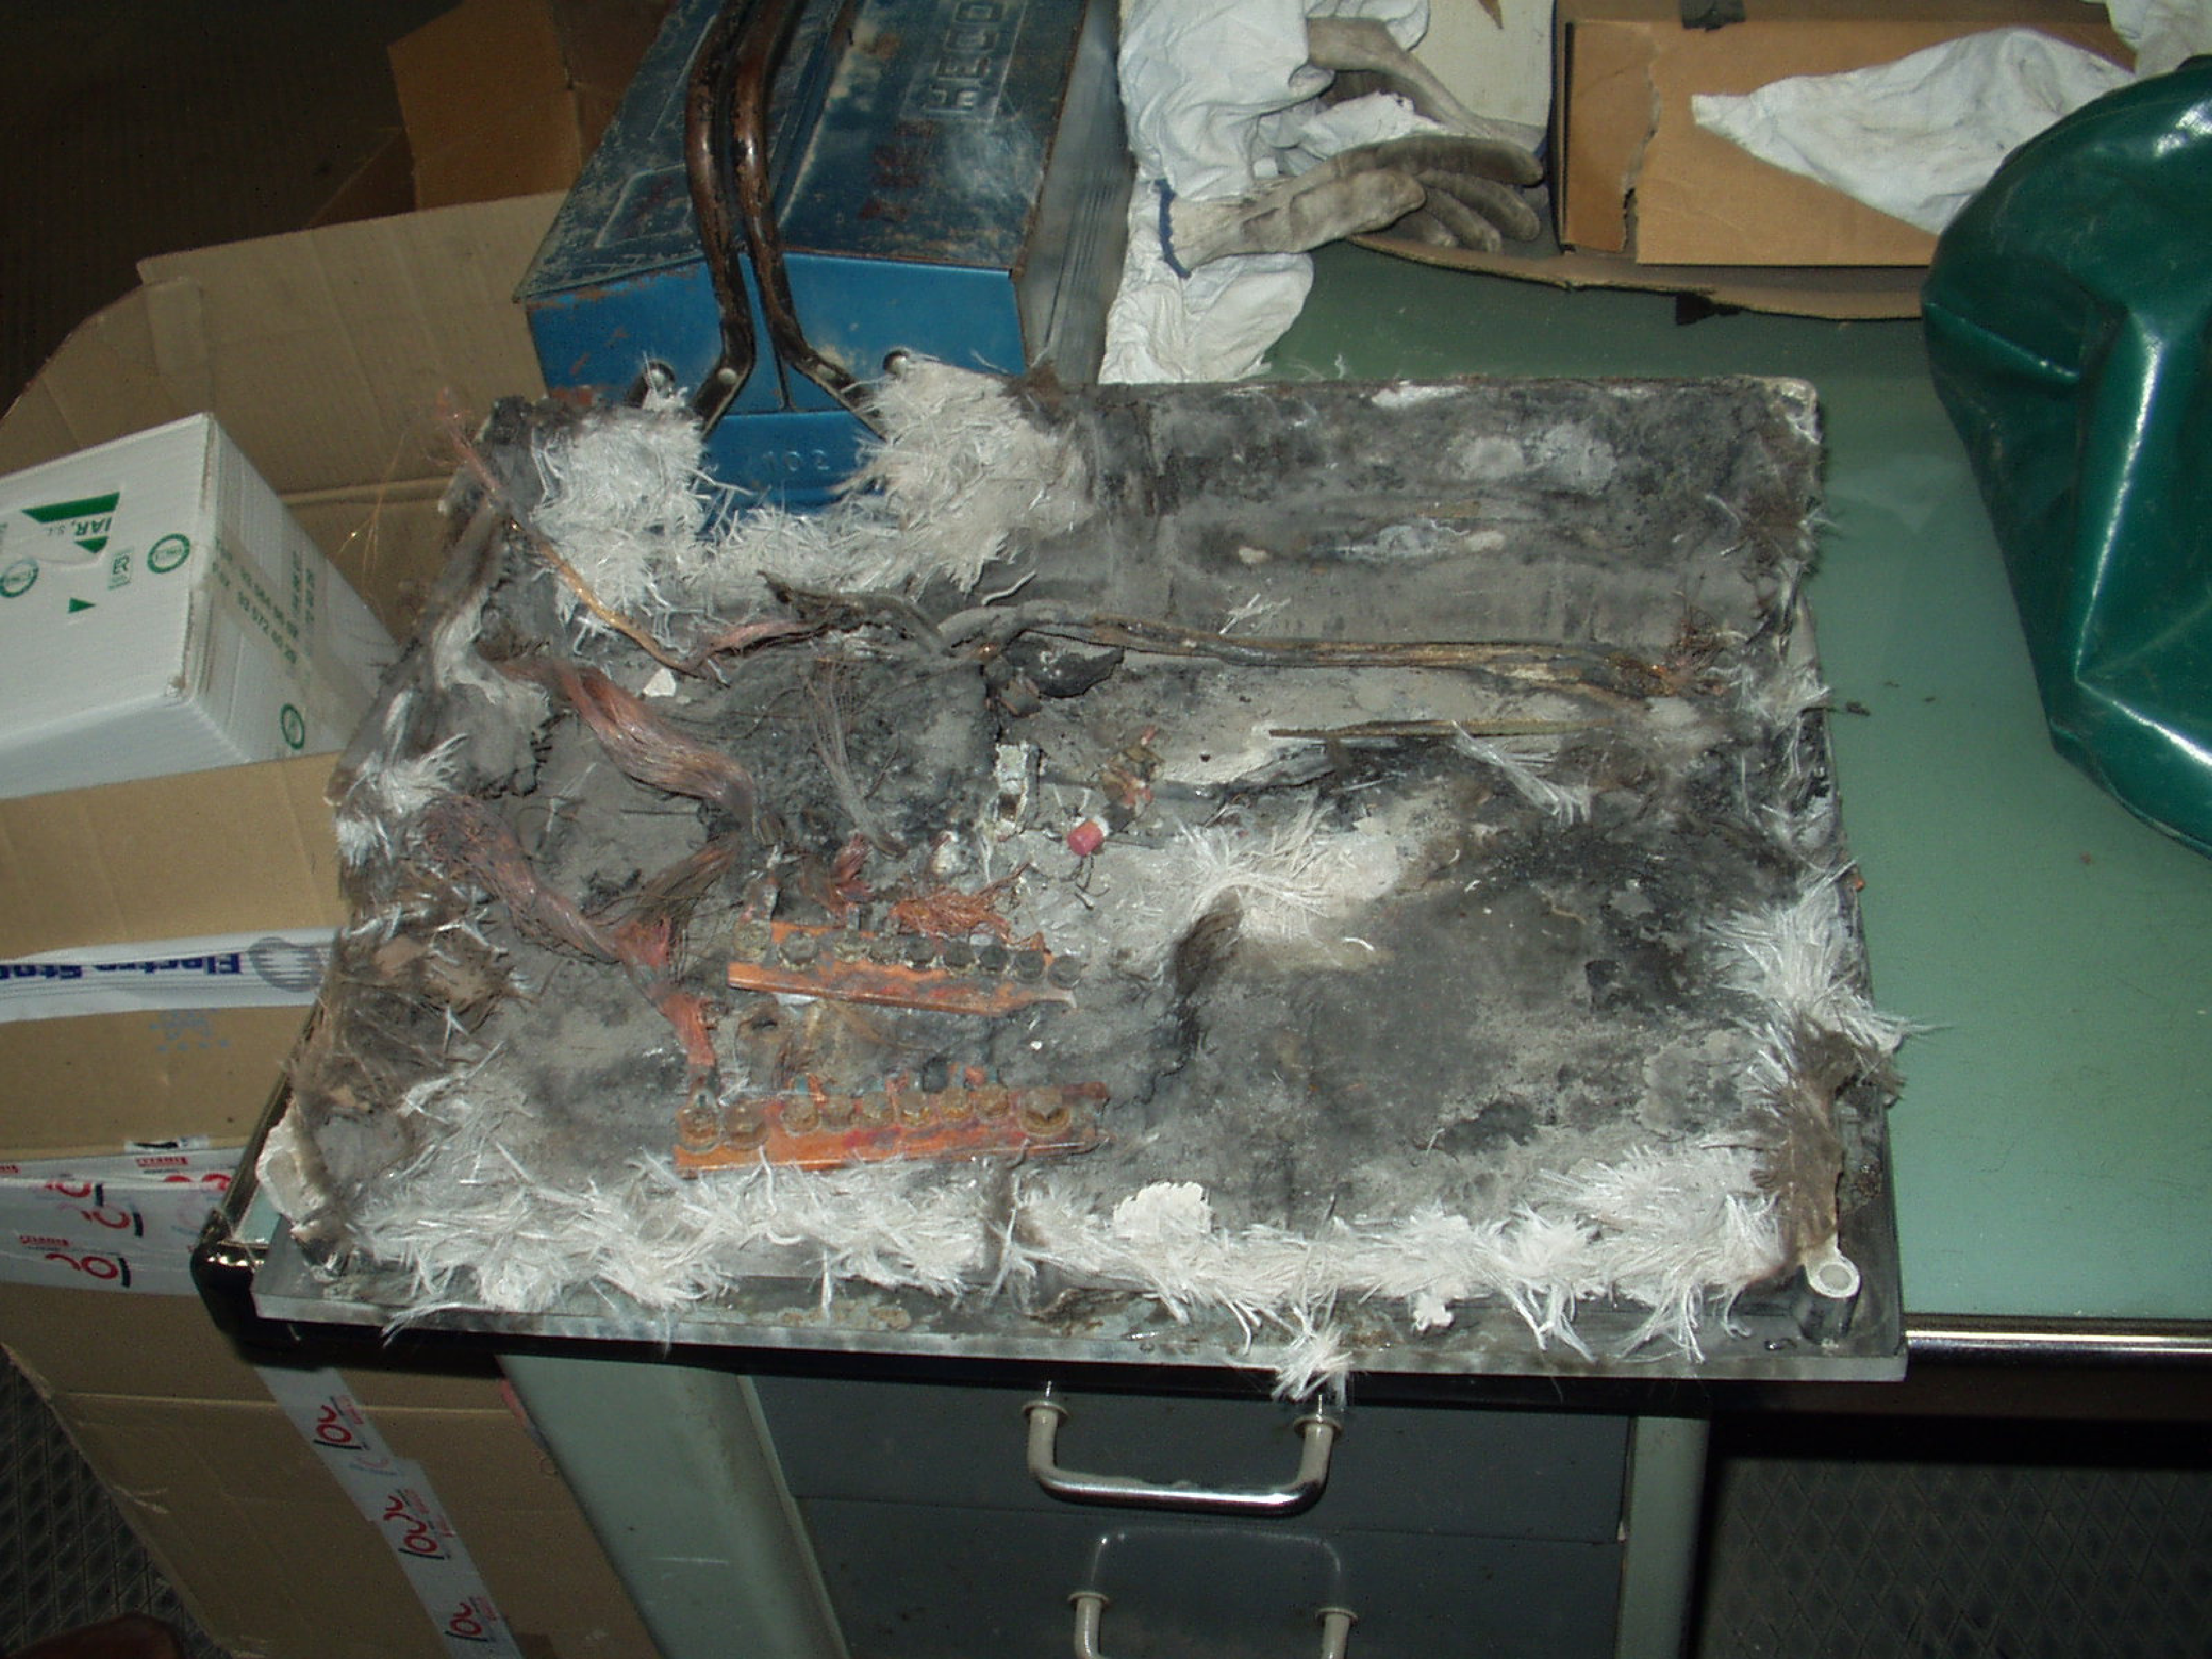
\includegraphics[scale=0.1]{../figs/CajaForumDestruida}
\end{centering}

\caption{Efectos del funcionamiento de un diseño defectuoso de una caja de
protecciones que incluye varistores.\label{fig:EfectosVaristor}}

\end{figure}



\section{Elementos de protección}

A continuación se describen los diferentes elementos que son necesarios
para acometer las tareas de protección reseñadas en los puntos anteriores.


\subsection{Protecciones en DC}


\subsubsection{Cortocircuitos}

El cortocircuito es un punto de trabajo no peligroso para el generador
fotovoltaico. Puede, sin embargo, ser perjudicial para el inversor.
Como medio de protección se recomienda incluir fusibles en cada polo%
\footnote{Para instalaciones fotovoltaicas son de uso común los fusibles de
tipo gG normalizados según la norma EN 60269.%
}. Por otra parte, el portafusible asociado sirve como elemento de
seccionamiento, facilitando las tareas de mantenimiento. Aunque el
cortocircuito no sea peligroso para el generador, su establecimiento
o extinción pueden ocasionar fácilmente un arco eléctrico si la maniobra
no se realiza con suficiente celeridad. De ahí que el seccionamiento
de parte del generador empleando los portafusibles deba realizarse
exclusivamente cuando el inversor se encuentra en modo de parada. 

Por otra parte, para evitar cortocircuitos ocasionados por eventuales
pérdidas de aislamiento en cables, es recomendable la conducción separada
del positivo y del negativo. Esta recomendación debe realizarse de
forma que el área efectiva ante tormentas eléctricas siga siendo la
mínima posible.

La elección de los fusibles se realiza mediante las ecuaciones \ref{eq:InDispositivoProteccion}
y \ref{eq:IntensidadAdmisibleConductor}:

\begin{eqnarray}
I_{B} & < & I_{n}<I_{z}\label{eq:InDispositivoProteccion}\\
I_{2} & < & 1.45\cdot I_{z}\label{eq:IntensidadAdmisibleConductor}\end{eqnarray}
siendo $I_{B}$ la intensidad de diseño de la línea, $I_{n}$ la intensidad
nominal del dispositivo de protección, $I_{z}$ la intensidad admisible
por el conductor e $I_{2}$ la intensidad que asegura efectivamente
el funcionamiento del dispositivo de protección.  \nomenclature[Ib]{$I_{B}$}{Intensidad de diseño de una línea eléctrica}\nomenclature[In]{$I_{n}$}{Intensidad nominal del dispositivo de protección}\nomenclature[Iz]{$I_{z}$}{Intensidad admisible por un conductor}\nomenclature[I2]{$I_{2}$}{Intensidad que asegura efectivamente el funcionamiento del dispositivo de protección}
Para fusibles, normalmente $I_{2}=1.6\cdot I_{n}$. En instalaciones
fotovoltaicas suele emplearse la relación $I_{n}\geq1.25\cdot I_{sc}$
para evitar paradas innecesarias, siendo $I_{sc}$ la corriente de
cortocircuito de la rama asociada al fusible en cuestión.

En las instalaciones eléctricas convencionales es frecuente el empleo
de fusibles (y otros elementos de protección) en cascada con poder
de corte creciente en dirección al punto de conexión a red. Esta práctica
se basa en que, en la red convencional, la corriente de cortocircuito
es sustancialmente superior a la de operación. Sin embargo, su traslación
directa a los sistemas fotovoltaicos carece de sentido dada la similitud
entre ambas corrientes. Aunque puede defenderse su utilidad al permitir
el seccionamiento parcial del generador debe tenerse en cuenta que
esta funcionalidad la ofrece el portafusibles y no el fusible mismo. 


\subsubsection{Sobretensiones}

La entrada de los equipos electrónicos (inversores o reguladores)
está protegida mediante varistores, tal y como ha sido descrito en
el apartado de protección de equipos. El rango de la tensión de operación
está definido por la tensión en el punto de máxima potencia y tensión
de circuito abierto del generador fotovoltaico.

En la figura \ref{fig:Caja-de-protecci=0000F3n} se muestra un ejemplo
de una caja de protecciones situada a la salida de un generador fotovoltaico.
Incluye un conjunto de fusibles de rama tanto en el polo positivo
como en el negativo. A la salida del paralelo de estos fusibles se
han instalado tres varistores, uno para conectar el polo positivo
con tierra, otro para conectar el polo negativo con tierra y otro
tercero para interconectar los dos polos. Existen equipos comerciales
que incluyen los tres varistores interconectados.

%
\begin{figure}
\begin{centering}
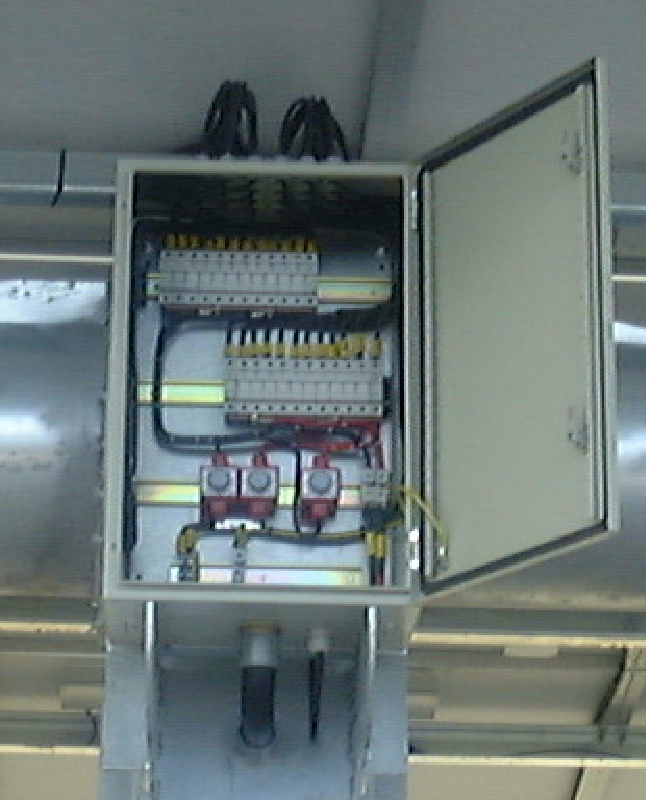
\includegraphics[scale=0.5]{../figs/CajaProteccionesPhotocampa}
\end{centering}

\caption[Caja de protección DC]{Caja de protección DC. Incluye dos fusibles por rama y varistores
entre polos y tierra.\label{fig:Caja-de-protecci=0000F3n}}

\end{figure}



\subsection{Protecciones en AC}


\subsubsection{Cortocircuitos y sobrecargas}

Según el RD 1663-2000 \cite{RealDecreto2000} es necesario incluir
un interruptor general manual, que será un interruptor magnetotérmico
omnipolar. Este interruptor, que se ubica en el cuadro de contadores
de la instalación fotovoltaica, será accesible sólo a la empresa distribuidora,
con objeto de poder realizar la desconexión manual, que permita la
realización, de forma segura, de labores de mantenimiento en la red
de la compañía eléctrica. Esta inaccesibilidad obliga a introducir
un segundo magnetotérmico omnipolar en la instalación, de menor intensidad
nominal, que será el que realmente proteja a la instalación AC de
las sobrecargas y cortocircuitos. Este segundo magnetotérmico actuará
antes que el interruptor general manual, salvo cortocircuitos de cierta
importancia provenientes de la red de la compañía. Asimismo, con el
fin de dar cierta independencia a las líneas propias de cada inversor,
se suele incluir un interruptor magnetotérmico de menor corriente
para cada inversor.

Se recomienda el empleo de magnetotérmicos tipo C, los utilizados
cuando no existen corrientes de arranque de consumo elevadas, cumpliendo
las ecuaciones \ref{eq:InDispositivoProteccion} y \ref{eq:IntensidadAdmisibleConductor},
junto con la relación $I_{2}=1.45\cdot I_{n}$, característica de
los interruptores magnetotérmicos normalizados.


\subsubsection{Fallos a tierra }

La instalación contará con un interruptor diferencial de sensibilidad
adecuada%
\footnote{En entornos industriales se admiten interruptores con sensibilidad
de $\SI{300}{\milli\ampere}$, mientras que para instalaciones domésticas
este valor se reduce a $\SI{30}{\milli\ampere}$.%
} en la parte de corriente alterna, para proteger de derivaciones en
este circuito. Con el fin de que sólo actúe por fallos a tierra, será
de una corriente asignada superior a la del magnetotérmico de protección. 

Para comprender dónde debe ser ubicado este interruptor, es necesario
recordar su funcionamiento. Un interruptor diferencial está basado en
un toroide que enlaza a todos los conductores. Si existe una corriente
de defecto, la corriente en cada conductor es diferente (figura
\ref{fig:FuncionamientoDiferencial}).  La corriente de defecto
circulará por tierra hasta alcanzar un camino de entrada al
circuito. En redes de distribución pública, donde el esquema de
conexión a tierra es TT, este camino de entrada se encuentra en la
puesta a tierra del neutro del centro de transformación. 

Supongamos ahora que se coloca un interruptor diferencial (simbolizado
en la figura \ref{fig:FuncionamientoDiferencial} por un círculo) a la
izquierda del fallo a tierra. En esta posición la corriente que
circula por los dos conductores es la misma, el interruptor
diferencial no detectará ninguna anomalía y no cortará el
circuito. Sin embargo, si el interruptor estuviese situado entre el
fallo y la puesta a tierra del centro de transformación, detectaría el
defecto dado que, en ese punto, la corriente que circula por cada
conductor es diferente. Por tanto, el diferencial \emph{no} protege el
tramo comprendido entre él y el centro de transformación. 

Es así que, para proteger la mayor longitud de circuito posible, la
ubicación del interruptor diferencial debe estar lo más cerca posible
del punto de conexión con la red eléctrica. En otras palabras, es un
error situar el interruptor diferencial justo en la salida de los
inversores, dado que todo el tramo entre ese punto y la conexión con
la red quedará desprotegido.

%
\begin{figure}
\begin{centering}
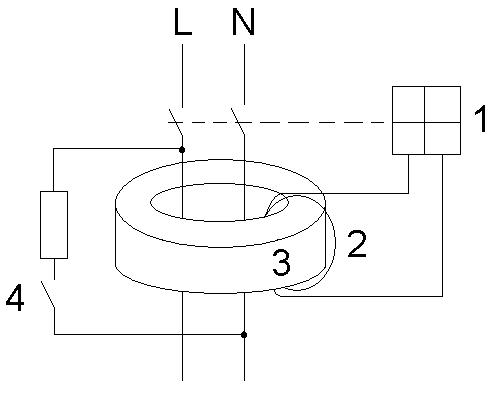
\includegraphics[scale=0.68]{../figs/InterruptorDiferencial}
\end{centering}

\caption{Funcionamiento de un interruptor diferencial.\label{fig:FuncionamientoDiferencial}}

\end{figure}


Por otra parte, es importante tener en cuenta que, al estar basado
en la ley de Faraday (fuerza electromotriz creada por un flujo magnético
\emph{variable}), no funciona en circuitos de corriente continua%
\footnote{Como anécdota, el RD 1663/2000 \cite{RealDecreto2000} ocasiona más
de un quebradero de cabeza al incluir en su artículo 11 el requerimiento
de incorporar un {}``interruptor automático diferencial, con el fin
de proteger a las personas en el caso de derivación de algún elemento
de la parte continua de la instalación''%
}. 


\subsubsection{Puesta a tierra}

Según el RD1663/2000 \cite{RealDecreto2000}, en que se fijan las
condiciones técnicas para la conexión de instalaciones fotovoltaicas
a la red, la puesta a tierra se realizará de forma que no altere la
de la compañía eléctrica distribuidora, con el fin de no transmitir
defectos a la misma. Asimismo, las masas de la instalación fotovoltaica
estarán conectadas a una tierra independiente de la del neutro de
la empresa distribuidora.


\subsection{Cableado}

La elección de la sección de cableado en sistemas fotovoltaicos se
basa principalmente en dos criterios: el térmico y el de la caída de
tensión. Ambos se deben a la resistencia ofrecida por el cable.  El
primero está relacionado con el efecto Joule, que supone una emisión
de calor que debe quedar por debajo de la soportada por el cable.  El
segundo tiene en cuenta la caída de tensión debida al paso de
corriente a través de la resistencia equivalente del cable.

Para calcular la sección necesaria según el criterio de caída de
tensión son aplicables las siguientes ecuaciones\footnote{En las ecuaciones se ha despreciado la inductancia de los
  cables, se ha considerado que el inversor trabaja con factor de
  potencia unidad,
  $\cos(\phi)=1$\nomenclature[cosphi]{$\cos(\phi)$}{Factor de potencia
    de una instalación eléctrica}, y se supone que el material
  conductor empleado es el cobre. %
} para los tramos de
corriente continua ($S_{dc}$), para el tramo ente
inversor y punto de conexión a red en sistemas monofásicos ($S_{1ac}$), y para sistemas trifásicos ($S_{3ac}$).

\[
  \begin{aligned}
    S_{dc} & = & \frac{2 \cdot L_{dc}\cdot I_{dc}}{\gamma_\theta \cdot \Delta V_{dc}}\\
    S_{1ac} & = & \frac{2\cdot L_{1ac}\cdot I_{1ac}}{\gamma_\theta \cdot \Delta V_{1ac}}\\
    S_{3ac} & = & \frac{\sqrt{3} \cdot L_{3ac}\cdot I_{3ac}}{\gamma_\theta \cdot \Delta V_{3ac}}
  \end{aligned}
\]

siendo $S_{dc}$ la sección de los conductores de corriente continua,
$L_{dc}$ la distancia a cubrir con un circuito de corriente continua
(el factor 2 tiene en cuenta que se necesitan dos conductores para
este circuito), $\gamma_\theta$ la conductividad del conductor a una temperatura
de operación determinada\footnote{La conductividad del cobre a 20ºC de
  temperatura de operación es $\gamma_{20} =\SI{56}{\meter\per\ohm\per\milli\meter\squared}$ mientras que a 70ºC es
$\gamma_{70} = \SI{48}{\meter\per\ohm\per\milli\meter\squared}$.},
$I_{dc}$ la corriente nominal (habitualmente la del punto MPP) que
circula por el circuito de corriente continua, y $\Delta V_{dc}$ la
caída de tensión existente entre la entrada y la salida del circuito
de corriente continua. La nomenclatura es similar en las otras dos
ecuaciones.

\nomenclature[Sdc]{$S_{dc}$}{Sección de
  un conductor de corriente continúa}
\nomenclature[S1ac]{$S_{1ac}$}{Sección de un conductor de corriente
  alterna monofásica}
\nomenclature[S3ac]{$S_{3ac}$}{Sección de un
  conductor de corriente alterna trifásica}
\nomenclature[ldc]{$L_{dc}$}{Distancia a cubrir con circuito de
  corriente continúa}
\nomenclature[l1ac]{$L_{1ac}$}{Distancia a
  cubrir con un un circuito de corriente alterna monofásica}
\nomenclature[l3ac]{$L_{3ac}$}{Distancia a cubrir con un circuito de
  corriente alterna trifásica}
\nomenclature[DeltaVdc]{$\Delta V_{dc}$}{Caida de tensión en un
  circuito de corriente continua}
\nomenclature[DeltaV1ac]{$\Delta V_{1ac}$}{Caida de tensión en un
  circuito de corriente alterna monofásica}
\nomenclature[DeltaV3ac]{$\Delta V_{3ac}$}{Caida de tensión en un
  circuito de corriente alterna trifásica}
\nomenclature[gamma_theta]{$\gamma_\theta$}{Conductividad de un conductor a una temperatura de operación determinada}

Según el apartado 5 de la ITC-BT-40, la caída máxima de tensión de la
tensión nominal entre el generador y el punto de interconexión a la
Red de Distribución Pública o a la instalación interior, no será
superior al $\SI{1.5}{\percent}$ para la intensidad nominal.
Habitualmente se aplica este mismo porcentaje de forma separada para
los circuitos de continua y de alterna, teniendo en cuenta que cada
zona (DC y AC) tiene su propia tensión nominal, tal y como se
especifica en las anteriores ecuaciones.

Además, hay que tener en cuenta que éste es un requisito que afecta a la
totalidad del circuito: cuando un circuito está dividido en varios
tramos (por ejemplo, por el uso de cajas de paralelos), la caída de
tensión total del circuito es la suma de las respectivas caídas en cada uno de los
tramos, y es esta suma a la que aplica el porcentaje anterior. Al
existir dos tramos y una única condición existe un grado de libertad
que permite fijar la sección de uno de los tramos u optimizar el
volumen total de conductor empleado (vease el ejercicio
\ref{EjercicioCableado})

Por ejemplo, en una instalación que conduce $\SI{75}{\ampere}$ a la
salida de un inversor trifásico, situado este a $\SI{100}{\meter}$ de
la conexión a red, se deberá utilizar un cable de sección:

\[
  S=\frac{\sqrt{3} \cdot 0.021 \cdot100\cdot75}{\SI{1.5}{\percent}\cdot400}=\SI{45.46}{\milli\meter\squared}
\]

Dado que la sección de los cables está normalizada, se deberá optar
por la sección inmediatamente superior, y por tanto la conexión del
inversor a la red se realizará con tres cables de sección
$S=\SI{50}{\milli\meter\squared}$.

Con este resultado, es necesario comprobar el cumplimiento del
criterio térmico. Según el apartado 5 de la ITC-BT-40, el cable debe
ser dimensionado para una intensidad no inferior al $125\%$ de la
máxima intensidad del generador.

En la zona de corriente de continua esta máxima intensidad se
corresponde con la corriente de cortocircuito del circuito en
análisis. Para la sección obtenida con el criterio de caída de
tensión, el valor $1.25 \cdot I_{sc}$ debe ser inferior a la
intensidad máxima admisible del cable para sus condiciones de
servicio.

Las tablas de la ITC-BT-07, recogen valores de intensidad máxima
admisible para el conjunto de secciones normalizadas para diferentes
conductores (cobre y aluminio), aislamiento (XLPE, EPR y PVC) y tipo
de instalación (enterrados, al aire, etc.). Además, existen diversos
factores de corrección dependiendo de la temperatura ambiente, de las
condiciones del terreno, de la agrupación de los cables, etc.

En general, debido a la combinación de distancias grandes y corrientes
de bajo valor, las secciones que resultan del criterio de caída de
tensión aplicado a los sistemas fotovoltaicos son capaces de conducir
la corriente del sistema, salvo en conexiones de corta longitud.

Para más detalles sobre el proceso de cálculo, se invita al lector a
repasar el ejercicio \ref{EjercicioCableado} y a la lectura del Anexo
2 a las Guías de Aplicación del
REBT\footnote{\url{www.f2i2.net/documentos/lsi/rbt/guias/guia_bt_anexo_2_sep03R1.pdf}}





%%% Local Variables:
%%% mode: LaTex
%%% TeX-master: "ESF.tex"
%%% End: 
